% Tokenization pipeline: compact version for NeurIPS
\documentclass[border=6pt]{standalone}
\usepackage{tikz}
\usepackage{amsmath,amssymb}
\usetikzlibrary{arrows.meta,positioning,shapes.geometric,fit,calc,
    decorations.pathmorphing,decorations.pathreplacing,backgrounds}

% Forgis brand colors — academic palette for white-background figures
% Source: color_schema.json
%
% Usage: % Forgis brand colors — academic palette for white-background figures
% Source: color_schema.json
%
% Usage: % Forgis brand colors — academic palette for white-background figures
% Source: color_schema.json
%
% Usage: \input{colors.tex} in each standalone figure .tex file.
% All figures MUST use only these colors. No inline hex.

% Brand primaries
\definecolor{ctiger}{HTML}{FF5A00}       % Primary accent (Forgis orange)
\definecolor{cfire}{HTML}{FF4D00}        % Critical
\definecolor{cflicker}{HTML}{DC4B07}     % Secondary accent
\definecolor{csteel}{HTML}{878F92}       % Muted neutral
\definecolor{cgunmetal}{HTML}{122128}    % Dark text

% Academic derived palette
\definecolor{cprimary}{HTML}{FF5A00}     % = tiger
\definecolor{cprimarylight}{HTML}{FF8C42}
\definecolor{cprimarybg}{HTML}{FFF0E6}
\definecolor{csecondary}{HTML}{2B6CB0}   % Complementary blue
\definecolor{csecondarylight}{HTML}{4A90D9}
\definecolor{csecondarybg}{HTML}{E8F0FA}
\definecolor{caccent}{HTML}{2D8A6E}      % Teal
\definecolor{caccentlight}{HTML}{5BB89A}
\definecolor{caccentbg}{HTML}{E6F5F0}
\definecolor{chighlight}{HTML}{DC4B07}   % = flicker
\definecolor{chighlightbg}{HTML}{FDEDE6}
\definecolor{ctextdark}{HTML}{122128}    % = gunmetal
\definecolor{ctextmid}{HTML}{878F92}     % = steel
\definecolor{ctextlight}{HTML}{B0B7BA}
\definecolor{cborder}{HTML}{D1D5D8}
\definecolor{cbgwarm}{HTML}{FFF8F2}
\definecolor{cbgcool}{HTML}{F4F7FA}
 in each standalone figure .tex file.
% All figures MUST use only these colors. No inline hex.

% Brand primaries
\definecolor{ctiger}{HTML}{FF5A00}       % Primary accent (Forgis orange)
\definecolor{cfire}{HTML}{FF4D00}        % Critical
\definecolor{cflicker}{HTML}{DC4B07}     % Secondary accent
\definecolor{csteel}{HTML}{878F92}       % Muted neutral
\definecolor{cgunmetal}{HTML}{122128}    % Dark text

% Academic derived palette
\definecolor{cprimary}{HTML}{FF5A00}     % = tiger
\definecolor{cprimarylight}{HTML}{FF8C42}
\definecolor{cprimarybg}{HTML}{FFF0E6}
\definecolor{csecondary}{HTML}{2B6CB0}   % Complementary blue
\definecolor{csecondarylight}{HTML}{4A90D9}
\definecolor{csecondarybg}{HTML}{E8F0FA}
\definecolor{caccent}{HTML}{2D8A6E}      % Teal
\definecolor{caccentlight}{HTML}{5BB89A}
\definecolor{caccentbg}{HTML}{E6F5F0}
\definecolor{chighlight}{HTML}{DC4B07}   % = flicker
\definecolor{chighlightbg}{HTML}{FDEDE6}
\definecolor{ctextdark}{HTML}{122128}    % = gunmetal
\definecolor{ctextmid}{HTML}{878F92}     % = steel
\definecolor{ctextlight}{HTML}{B0B7BA}
\definecolor{cborder}{HTML}{D1D5D8}
\definecolor{cbgwarm}{HTML}{FFF8F2}
\definecolor{cbgcool}{HTML}{F4F7FA}
 in each standalone figure .tex file.
% All figures MUST use only these colors. No inline hex.

% Brand primaries
\definecolor{ctiger}{HTML}{FF5A00}       % Primary accent (Forgis orange)
\definecolor{cfire}{HTML}{FF4D00}        % Critical
\definecolor{cflicker}{HTML}{DC4B07}     % Secondary accent
\definecolor{csteel}{HTML}{878F92}       % Muted neutral
\definecolor{cgunmetal}{HTML}{122128}    % Dark text

% Academic derived palette
\definecolor{cprimary}{HTML}{FF5A00}     % = tiger
\definecolor{cprimarylight}{HTML}{FF8C42}
\definecolor{cprimarybg}{HTML}{FFF0E6}
\definecolor{csecondary}{HTML}{2B6CB0}   % Complementary blue
\definecolor{csecondarylight}{HTML}{4A90D9}
\definecolor{csecondarybg}{HTML}{E8F0FA}
\definecolor{caccent}{HTML}{2D8A6E}      % Teal
\definecolor{caccentlight}{HTML}{5BB89A}
\definecolor{caccentbg}{HTML}{E6F5F0}
\definecolor{chighlight}{HTML}{DC4B07}   % = flicker
\definecolor{chighlightbg}{HTML}{FDEDE6}
\definecolor{ctextdark}{HTML}{122128}    % = gunmetal
\definecolor{ctextmid}{HTML}{878F92}     % = steel
\definecolor{ctextlight}{HTML}{B0B7BA}
\definecolor{cborder}{HTML}{D1D5D8}
\definecolor{cbgwarm}{HTML}{FFF8F2}
\definecolor{cbgcool}{HTML}{F4F7FA}


\begin{document}
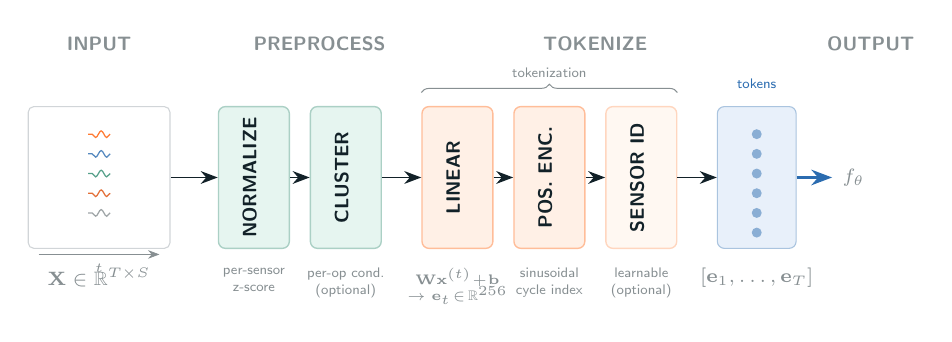
\begin{tikzpicture}[
    >=Stealth,
    font=\sffamily\small,
    dataarrow/.style={->,line width=0.7pt,ctextdark},
    sechead/.style={font=\sffamily\scriptsize\bfseries,text=ctextmid},
    annot/.style={font=\sffamily\scriptsize,text=ctextmid},
    tallblock/.style={
        rounded corners=2.5pt, line width=0.5pt,
        minimum height=1.8cm, minimum width=0.9cm,
        align=center, text=ctextdark, inner sep=2pt,
    },
]

% ============================================================
% SECTION HEADERS
% ============================================================
\node[sechead] at (0,2.5) {INPUT};
\node[sechead] at (2.8,2.5) {PREPROCESS};
\node[sechead] at (6.3,2.5) {TOKENIZE};
\node[sechead] at (9.8,2.5) {OUTPUT};

% ============================================================
% INPUT: Raw multivariate time series
% ============================================================
\node[rounded corners=2pt, draw=cborder, fill=white,
    minimum height=1.8cm, minimum width=1.8cm,
    inner sep=0pt] (signals) at (0,0.8) {};

\begin{scope}
    \clip ([xshift=2pt,yshift=2pt]signals.south west)
        rectangle ([xshift=-2pt,yshift=-2pt]signals.north east);
    \foreach \yoff/\col in {
        0.55/cprimary, 0.3/csecondary, 0.05/caccent,
        -0.2/chighlight, -0.45/ctextmid} {
        \draw[\col,line width=0.45pt,opacity=0.8,
              decorate,decoration={snake,amplitude=1.2pt,segment length=4pt}]
            ([xshift=4pt,yshift=\yoff cm]signals.center)
            -- ([xshift=-4pt,yshift=\yoff cm]signals.center);
    }
\end{scope}

\node[annot,below=0.12cm of signals] {$\mathbf{X}\in\mathbb{R}^{T\times S}$};

% Time arrow
\draw[->,line width=0.25pt,ctextmid]
    ([xshift=4pt,yshift=-2pt]signals.south west)
    -- ([xshift=-4pt,yshift=-2pt]signals.south east)
    node[midway,below=0pt,font=\sffamily\tiny,text=ctextmid] {$t$};

% ============================================================
% PREPROCESSING
% ============================================================

\node[tallblock, draw=caccent!40, fill=caccentbg,
    right=0.6cm of signals] (norm) {
    \rotatebox{90}{\scriptsize\textbf{NORMALIZE}}
};
\node[annot,below=0.12cm of norm,align=center] {
    {\tiny per-sensor}\\[-2pt]{\tiny z-score}
};
\draw[dataarrow] (signals.east) -- (norm.west);

\node[tallblock, draw=caccent!40, fill=caccentbg,
    right=0.25cm of norm] (cond) {
    \rotatebox{90}{\scriptsize\textbf{CLUSTER}}
};
\node[annot,below=0.12cm of cond,align=center] {
    {\tiny per-op cond.}\\[-2pt]{\tiny (optional)}
};
\draw[dataarrow] (norm.east) -- (cond.west);

% ============================================================
% TOKENIZATION
% ============================================================

\node[tallblock, draw=cprimary!40, fill=cprimarybg,
    right=0.5cm of cond] (proj) {
    \rotatebox{90}{\scriptsize\textbf{LINEAR}}
};
\node[annot,below=0.12cm of proj,align=center] {
    {\tiny $\mathbf{W}\mathbf{x}^{(t)}\!+\!\mathbf{b}$}\\[-2pt]
    {\tiny $\to\mathbf{e}_t\!\in\!\mathbb{R}^{256}$}
};
\draw[dataarrow] (cond.east) -- (proj.west);

\node[tallblock, draw=cprimary!40, fill=cprimarybg,
    right=0.25cm of proj] (pe) {
    \rotatebox{90}{\scriptsize\textbf{POS. ENC.}}
};
\node[annot,below=0.12cm of pe,align=center] {
    {\tiny sinusoidal}\\[-2pt]{\tiny cycle index}
};
\draw[dataarrow] (proj.east) -- (pe.west);

\node[tallblock, draw=cprimary!25, fill=cprimarybg!50,
    right=0.25cm of pe] (sid) {
    \rotatebox{90}{\scriptsize\textbf{SENSOR ID}}
};
\node[annot,below=0.12cm of sid,align=center] {
    {\tiny learnable}\\[-2pt]{\tiny (optional)}
};
\draw[dataarrow] (pe.east) -- (sid.west);

% Brace over tokenization blocks
\draw[decorate,decoration={brace,amplitude=3pt,raise=2pt},ctextmid,line width=0.35pt]
    ([yshift=0.1cm]proj.north west) -- ([yshift=0.1cm]sid.north east)
    node[midway,above=4pt,font=\sffamily\tiny,text=ctextmid] {tokenization};

% ============================================================
% OUTPUT
% ============================================================

\node[rounded corners=2.5pt, draw=csecondary!40, fill=csecondarybg,
    minimum height=1.8cm, minimum width=1.0cm,
    right=0.5cm of sid, align=center, inner sep=2pt] (out) {};

\foreach \y in {0.55,0.3,0.05,-0.2,-0.45,-0.7} {
    \fill[csecondary!55] ([yshift=\y cm]out.center) circle (1.8pt);
}

\node[annot,below=0.12cm of out] {$[\mathbf{e}_1,\ldots,\mathbf{e}_T]$};
\node[font=\sffamily\tiny,csecondary,above=0.1cm of out] {tokens};
\draw[dataarrow] (sid.east) -- (out.west);

% Arrow to encoder
\draw[->,line width=1.0pt,csecondary]
    (out.east) -- ++(0.45,0)
    node[right,annot] {$f_\theta$};

\end{tikzpicture}
\end{document}
